\documentclass[10pt, compress]{beamer}

\usetheme{amii}

\usepackage[scale=2]{ccicons}
\usepackage{booktabs}
\usepackage{minted}
\usepackage{tikz}

\usemintedstyle{trac}
\usetikzlibrary{arrows,automata,shapes.geometric,shapes.multipart}

\title{{\large Comparing Direct and Indirect Temporal-Difference Methods for Estimating the Variance of the Return}}
\subtitle{}
\date{\vspace{-0.5em}}
\author{Craig Sherstan, Dylan R. Ashley$^{*}$, Brendan Bennett$^{*}$, Kenny Young, \newline
        Adam White, Martha White, Richard S. Sutton}
\institute{Reinforcement Learning and Artificial Intelligence Laboratory, University of Alberta}

\begin{document}

\maketitle

\section{Background}

\begin{frame}{What is reinforcement learning?}
    Reinforcement learning considers an agent interacting with an environment:

    \begin{figure}
        \centering
        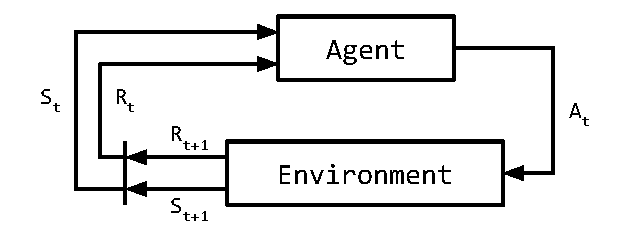
\includegraphics[height=8em]{{images/reinforcement_learning.pdf}}
    \end{figure}

    The function the agent uses to pick actions in states is known as the policy. Often the challenge is to find a "good" policy.
\end{frame}

\begin{frame}{What is a good policy?}\vspace{1em}
    In reinforcement learning the return is defined as follows:
    \begin{equation*}
        G_{\,t} = R_{\,t + 1} + \gamma_{\,t + 1} \,R_{\,t + 2} + \gamma_{\,t + 1} \,\gamma_{\,t + 2} \,R_{\,t + 3} + \ldots
    \end{equation*}

    Often we want to maximize the \alert{expected value} of the return. But "good" does depend on what we want.
\end{frame}

\begin{frame}{How can we learn it's expected value?}\vspace{1em}
    Temporal-difference (TD) methods have been fairly successful in tackling reinforcement learning problems so far. TD methods use predictions to update predictions.

    \vspace{1em}
    One of the most straightforward TD methods is TD($\lambda$):
    \begin{align*}
        \delta_{\,t} &= R_{\,t + 1} + \gamma_{\,t + 1} \,w_{\,t}^{\,T} \,x_{\,t + 1} - w_{\,t}^{\,T} \,x_{\,t} \\
        z_{\,t} &= \gamma_{\,t} \,\lambda_{\,t} \,z_{\,t - 1} + x_{\,t} \\
        w_{\,t + 1} &= w_{\,t} + \alpha_{\,t + 1} \,\delta_{\,t} \,z_{\,t} \\
    \end{align*}
\end{frame}

\begin{frame}{So what's this presentation about?}\vspace{1em}
    Recall what the return is:
    \begin{equation*}
        G_{\,t} = R_{\,t + 1} + \gamma_{\,t + 1} \,R_{\,t + 2} + \gamma_{\,t + 1} \,\gamma_{\,t + 2} \,R_{\,t + 3} + \ldots
    \end{equation*}

    We're not limited to learning only it's expected value. We could also learn more parts of its distribution such as its \alert{variance}.
\end{frame}

\section{Motivation}

\begin{frame}{Why might we want to learn its variance?}
    The variance might tell us things about the distribution that the expected value can't. Sometimes these things are \alert{interesting}. For example it could differentiate these two domains:

    \vspace{1em}
    \begin{figure}
        \centering
        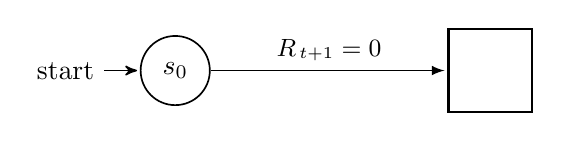
\begin{tikzpicture}[->,>=stealth',shorten >=1pt,auto,node distance=4cm,semithick]

            \tikzstyle{every state}=[draw=black,text=black]
            \tikzstyle{every text node part}=[align=center]
            \tikzstyle{terminal}=[regular polygon,regular polygon sides=4,thick,minimum size=1.5cm,draw=black]

            \node[initial,state] (0)              {$s_0$};
            \node[terminal]      (1) [right of=0] {};

            \small
            \draw[-latex]  (0) edge node [align=center,above] {\(R_{\,t + 1} = 0\)} (1);
        \end{tikzpicture}
    \end{figure}

    \begin{figure}
        \centering
        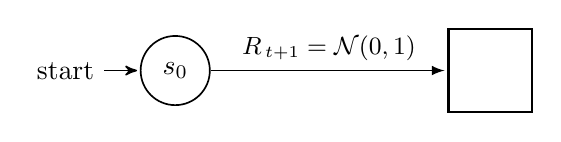
\begin{tikzpicture}[->,>=stealth',shorten >=1pt,auto,node distance=4cm,semithick]

            \tikzstyle{every state}=[draw=black,text=black]
            \tikzstyle{every text node part}=[align=center]
            \tikzstyle{terminal}=[regular polygon,regular polygon sides=4,thick,minimum size=1.5cm,draw=black]

            \node[initial,state] (0)              {$s_0$};
            \node[terminal]      (1) [right of=0] {};

            \small
            \draw[-latex]  (0) edge node [align=center,above] {\(R_{\,t + 1} = \mathcal{N}(0, 1)\)} (1);
        \end{tikzpicture}
    \end{figure}
\end{frame}

\begin{frame}{Any better reasons?}
    The variance can give us \alert{useful} information about the distribution. It can tell us how risky an action is to take in a state.

    \vspace{1em}
    Humans take risk into decisions and don't necessarily act in a way that maximizes the expected value.
\end{frame}

\begin{frame}{Anything else?}
    We can use an estimate of the variance to \alert{learn} how to learn. For example here is an algorithm that uses an estimate of the variance to tune $\lambda$ on the fly:

    \begin{figure}
        \centering
        \href{https://arxiv.org/abs/1607.00446}{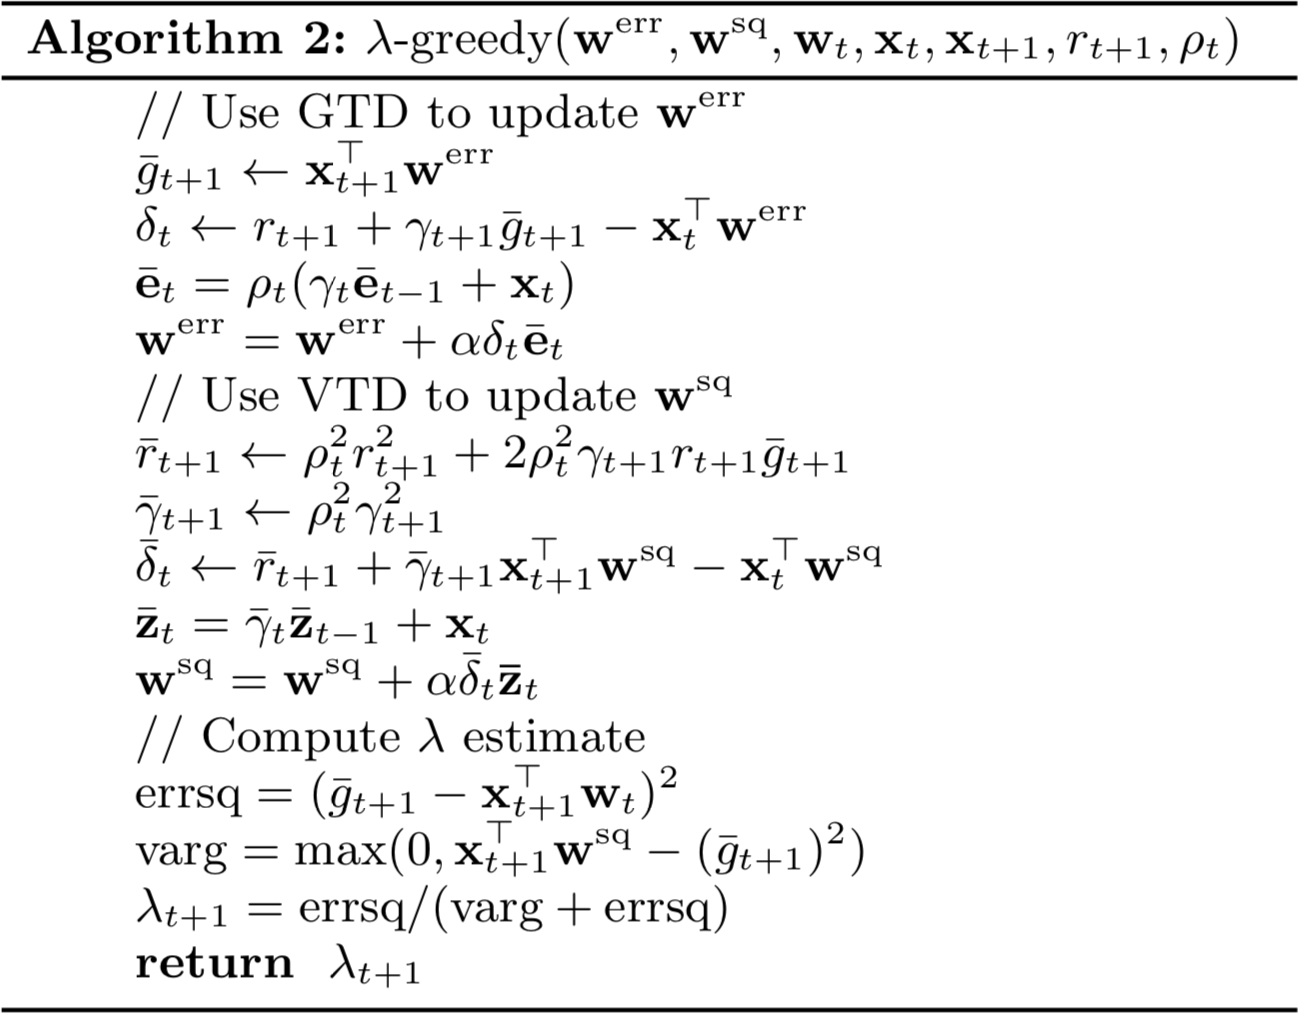
\includegraphics[height=15em]{{images/lambda_greedy.png}}}
    \end{figure}
\end{frame}

\section{Learning the Variance}

\begin{frame}{How can we learn its variance?}
    We can use this identity:
    \begin{equation*}
        Var(X) = \mathbb{E}\big[X^{\,2}\big] - \big(\mathbb{E}\big[X\big]\big)^2
    \end{equation*}

    If we are learning \(\mathbb{E}_{\pi} [G_{\,t} \,|\, S_{\,t} = s]\) then we can just learn \(\mathbb{E}_{\pi} [G_{\,t}^{\,2} \,|\, S_{\,t} = s]\) on the side and use both our estimates to try to estimate \(Var_{\pi}(G_{\,t} \,|\, S_{\,t} = s)\).
\end{frame}

\begin{frame}{What would this look like?}
   Using the identity \(Var(X) = \mathbb{E}\big[X^{\,2}\big] - \big(\mathbb{E}\big[X\big]\big)^2\) one can estimate the variance using the following structure:

    \vspace{1em}
    \begin{figure}
        \centering
        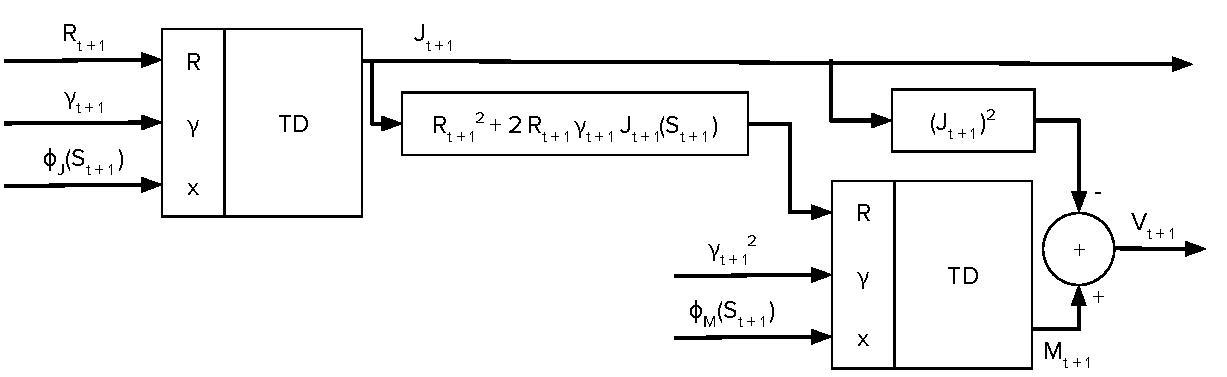
\includegraphics[height=8em]{{images/indirect.pdf}}
    \end{figure}
\end{frame}

\begin{frame}{Is there another way?}
    We can also use this identity:
    \begin{equation*}
        Var(X) = \mathbb{E}\big[\big(X - \mathbb{E}\big[X\big]\big)^{\,2}]
    \end{equation*}

    If we are learning \(\mathbb{E}_{\pi} [G_{\,t} \,|\, S_{\,t} = s]\) then we can approximate the variance using the following:
    \vspace{1em}
    \begin{equation*}
        Var_{\pi}(G_{\,t} \,|\, S_{\,t} = s) \approx \mathbb{E}_{\pi} \left[\delta_{\,t}^{\,2} + \sum\limits_{i \,= \,t + 1}^{\infty} \left(\delta_{\,i} \prod\limits_{j \,=\, t + 1}^{i} \gamma_{\,j} \,\right)^{2} \,\Bigg|\, S_{\,t} = s\right]
    \end{equation*}
\end{frame}

\begin{frame}{So how would this look?}
    Using the identity \(Var(X) = \mathbb{E}\big[\big(X - \mathbb{E}\big[X\big]\big)^{\,2}]\) one can estimate the variance using the following structure:

    \vspace{1em}
    \begin{figure}
        \centering
        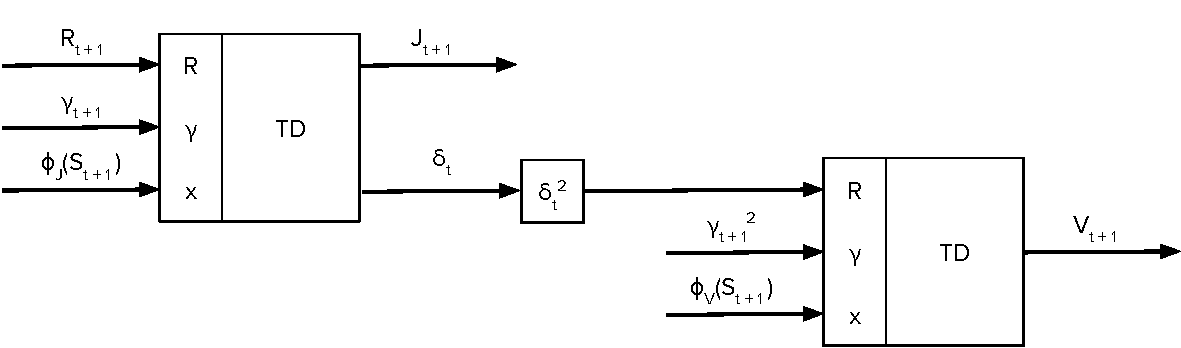
\includegraphics[height=7.277em]{{images/direct.pdf}}
    \end{figure}
\end{frame}

\begin{frame}{What would be the update equations for this?}
    Using TD($\lambda$) with $\overline{w}$ as the parameter vector for estimating the variance we obtain the following update equations:
    \vspace{1em}
    \begin{align*}
        \delta_{\,t} &= R_{\,t + 1} + \gamma_{\,t + 1} \,w_{\,t}^{\,T} \,x_{\,t + 1} - w_{\,t}^{\,T} \,x_{\,t} \\
        z_{\,t} &= \gamma_{\,t} \,\lambda_{\,t} \,z_{\,t - 1} + x_{\,t} \\
        w_{\,t + 1} &= w_{\,t} + \alpha_{\,t + 1} \,\delta_{\,t} \,z_{\,t} \\[1em]
        %
        \overline{\delta}_{\,t} &= \delta_{\,t}^{\,2} + \gamma_{\,t + 1}^{\,2} \,\overline{w}_{\,t}^{\,T} \,x_{\,t + 1} - \overline{w}_{\,t}^{\,T} \,x_{\,t} \\
        \overline{z}_{\,t} &= \gamma_{\,t}^{\,2} \,\overline{\lambda}_{\,t} \,\overline{z}_{\,t - 1} + x_{\,t} \\
        \overline{w}_{\,t + 1} &= \overline{w}_{\,t} + \overline{\alpha}_{\,t + 1} \,\overline{\delta}_{\,t} \,\overline{z}_{\,t}
    \end{align*}
\end{frame}

\begin{frame}{How do they compare visually?}
    \vspace{1em}
    \begin{figure}
        \flushleft
        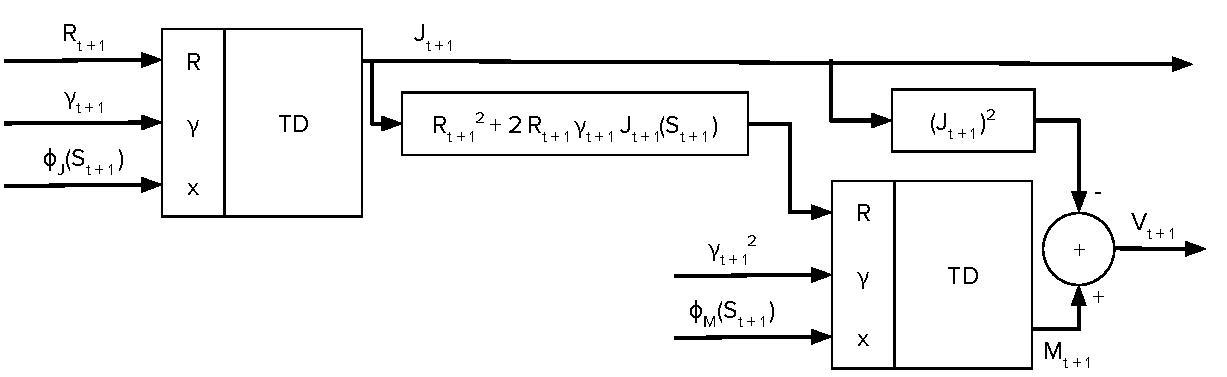
\includegraphics[height=8em]{{images/indirect.pdf}}
    \end{figure}
    \vspace{1em}
    \begin{figure}
        \flushleft
        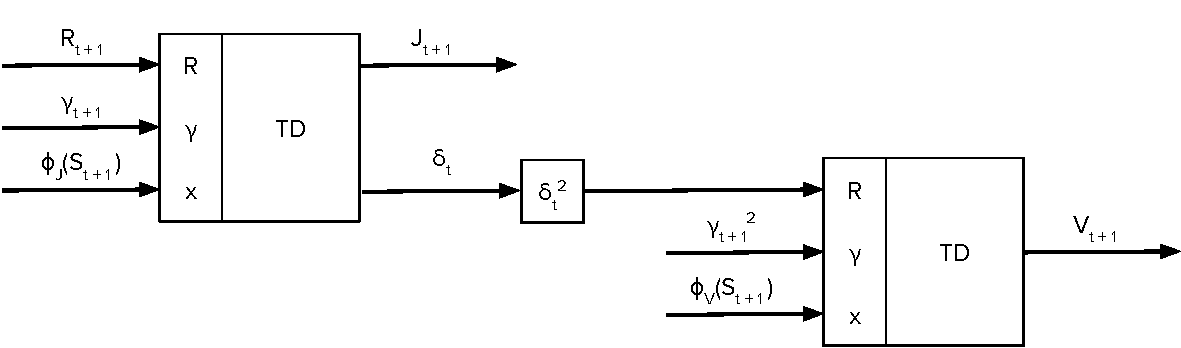
\includegraphics[height=7.277em]{{images/direct.pdf}}
    \end{figure}
\end{frame}

\section{Empirical Comparison}

\begin{frame}{What do we want to know?}\vspace{1em}
    Ideally we want to know if the direct method

    \begin{itemize}
        \item is faster or slower to converge than the indirect method,
        \item is more robust or less robust to differences in the value and variance learner, and
        \item performs better or worse under linear function approximation.
    \end{itemize}
\end{frame}

\begin{frame}{What is the simplest domain we can compare them on?}\vspace{1em}
    We begin by comparing them on the following simple Markov chain with gaussian rewards:

    \vspace{1em}
    \begin{figure}
        \hspace{-2.5em}\includegraphics[width=0.8\linewidth]{{images/chain/state_diagram.pdf}}
    \end{figure}
\end{frame}

\begin{frame}{How do they compare when \(\alpha = \overline{\alpha}\) ?}\vspace{1em}
    When \(\alpha = \overline{\alpha} = 0.001\) both perform roughly the same:

    \vspace{1em}
    \begin{figure}
        \hspace{-2.5em}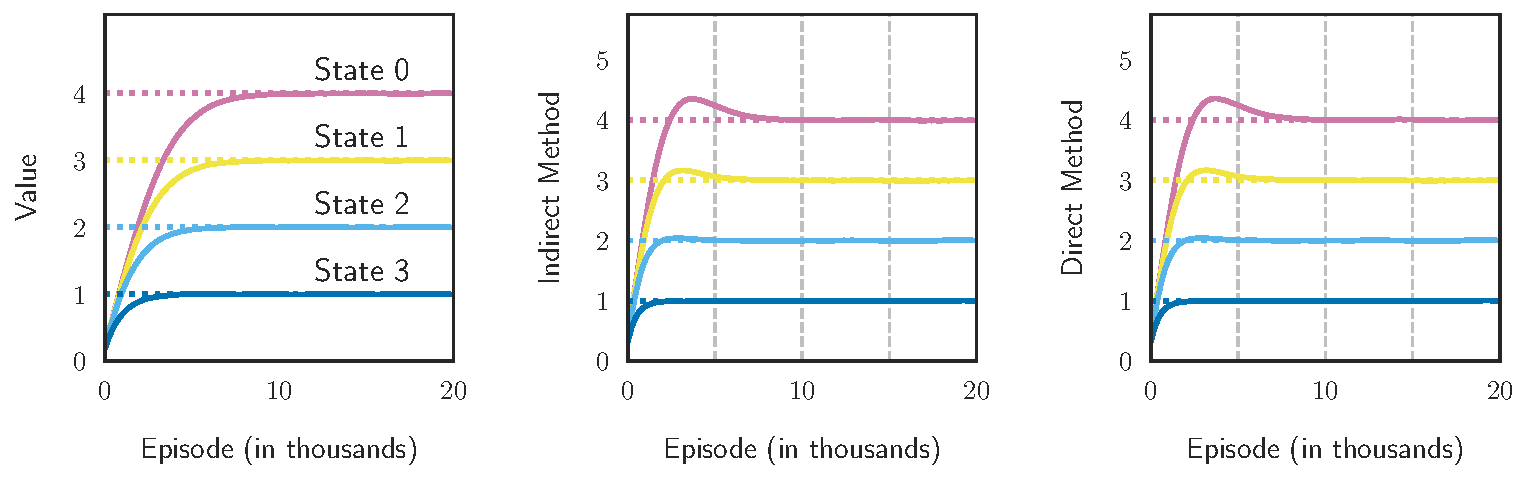
\includegraphics[width=0.9\linewidth]{{images/chain/same_step_size.pdf}}
    \end{figure}
\end{frame}

\begin{frame}{What about when \(\alpha > \overline{\alpha}\) ?}\vspace{1em}
    When \(\alpha = 0.01\) and \(\overline{\alpha} = 0.001\) the variance of the indirect method is higher:

    \vspace{1em}
    \begin{figure}
        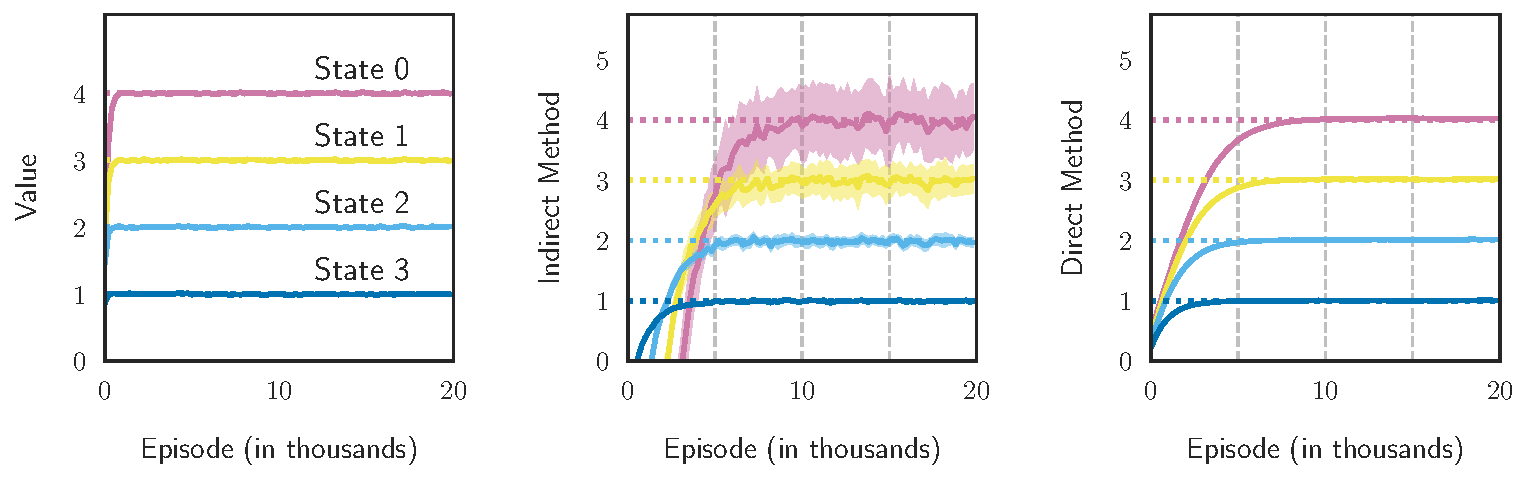
\includegraphics[width=0.9\linewidth]{{images/chain/value_step_size_greater.pdf}}
    \end{figure}
\end{frame}

\begin{frame}{So what about when \(\alpha < \overline{\alpha}\) ?}\vspace{1em}
    When \(\alpha = 0.001\) and \(\overline{\alpha} = 0.01\) the variance of the indirect method is higher and the direct method is more stable:

    \vspace{1em}
    \begin{figure}
        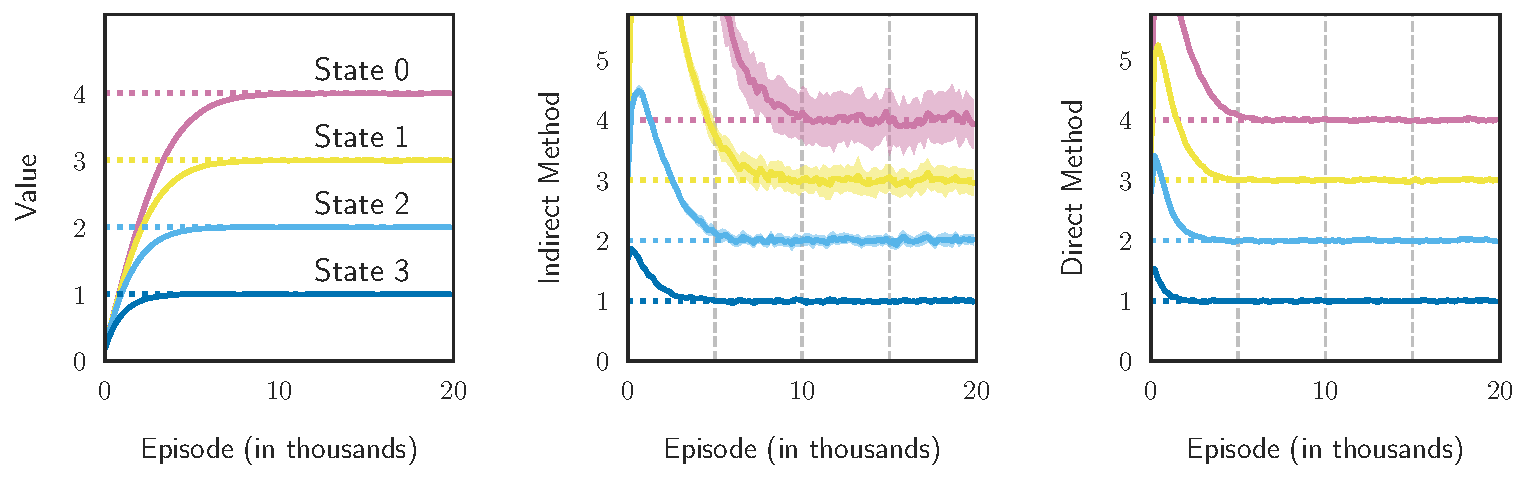
\includegraphics[width=0.9\linewidth]{{images/chain/variance_step_size_greater.pdf}}
    \end{figure}
\end{frame}

\begin{frame}{Does this result generalize?}\vspace{1em}
    In this domain we only see the two perform similarly when both step sizes are equal (note that the dotted line represents the indirect method and the solid line represents the direct method):

    \vspace{1em}
    \begin{figure}
        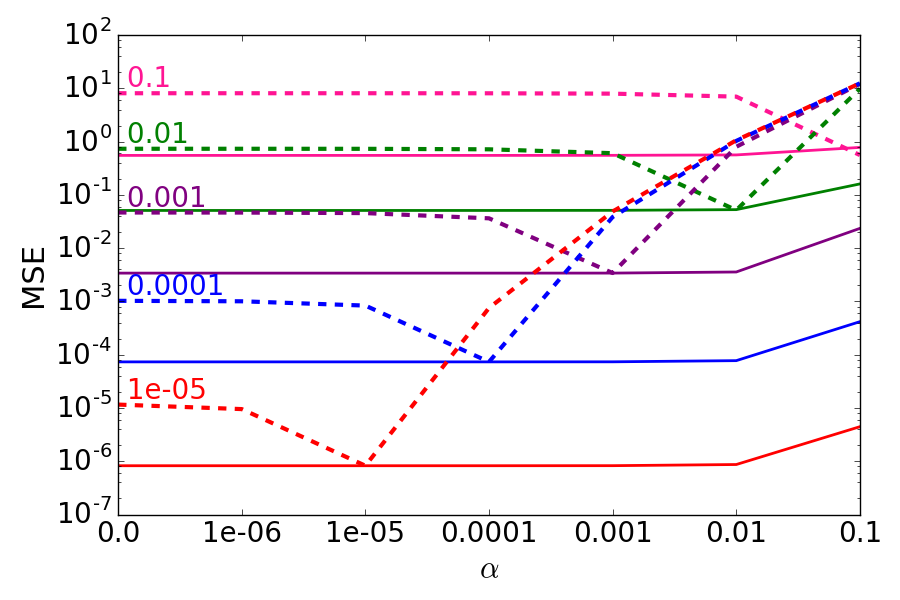
\includegraphics[width=0.7\linewidth]{{images/chain/sweep.png}}
    \end{figure}
\end{frame}

\begin{frame}{What about under function approximation?}\vspace{1em}
    We use the following domain previously used to evaluate the indirect method:

    \begin{figure}
        \hspace{-2.5em}\includegraphics[width=0.9\linewidth]{{images/random_walk/state_diagram.pdf}}
    \end{figure}

    For each state $s_{\,i}$ we use \(\phi(s_{\,i}) = [1, \,i / 30]^{\,T}\) for our value estimator and \(\phi_{\,2}(s_{\,i}) = [1, \,i / 30, \,(i / 30)^{\,2}]^{\,T}\) for our variance estimator.
\end{frame}

\begin{frame}{How do they perform on this domain?}\vspace{0.75em}
    Here the direct method vastly outperforms the indirect method:

    \vspace{0.5em}
    \begin{figure}
        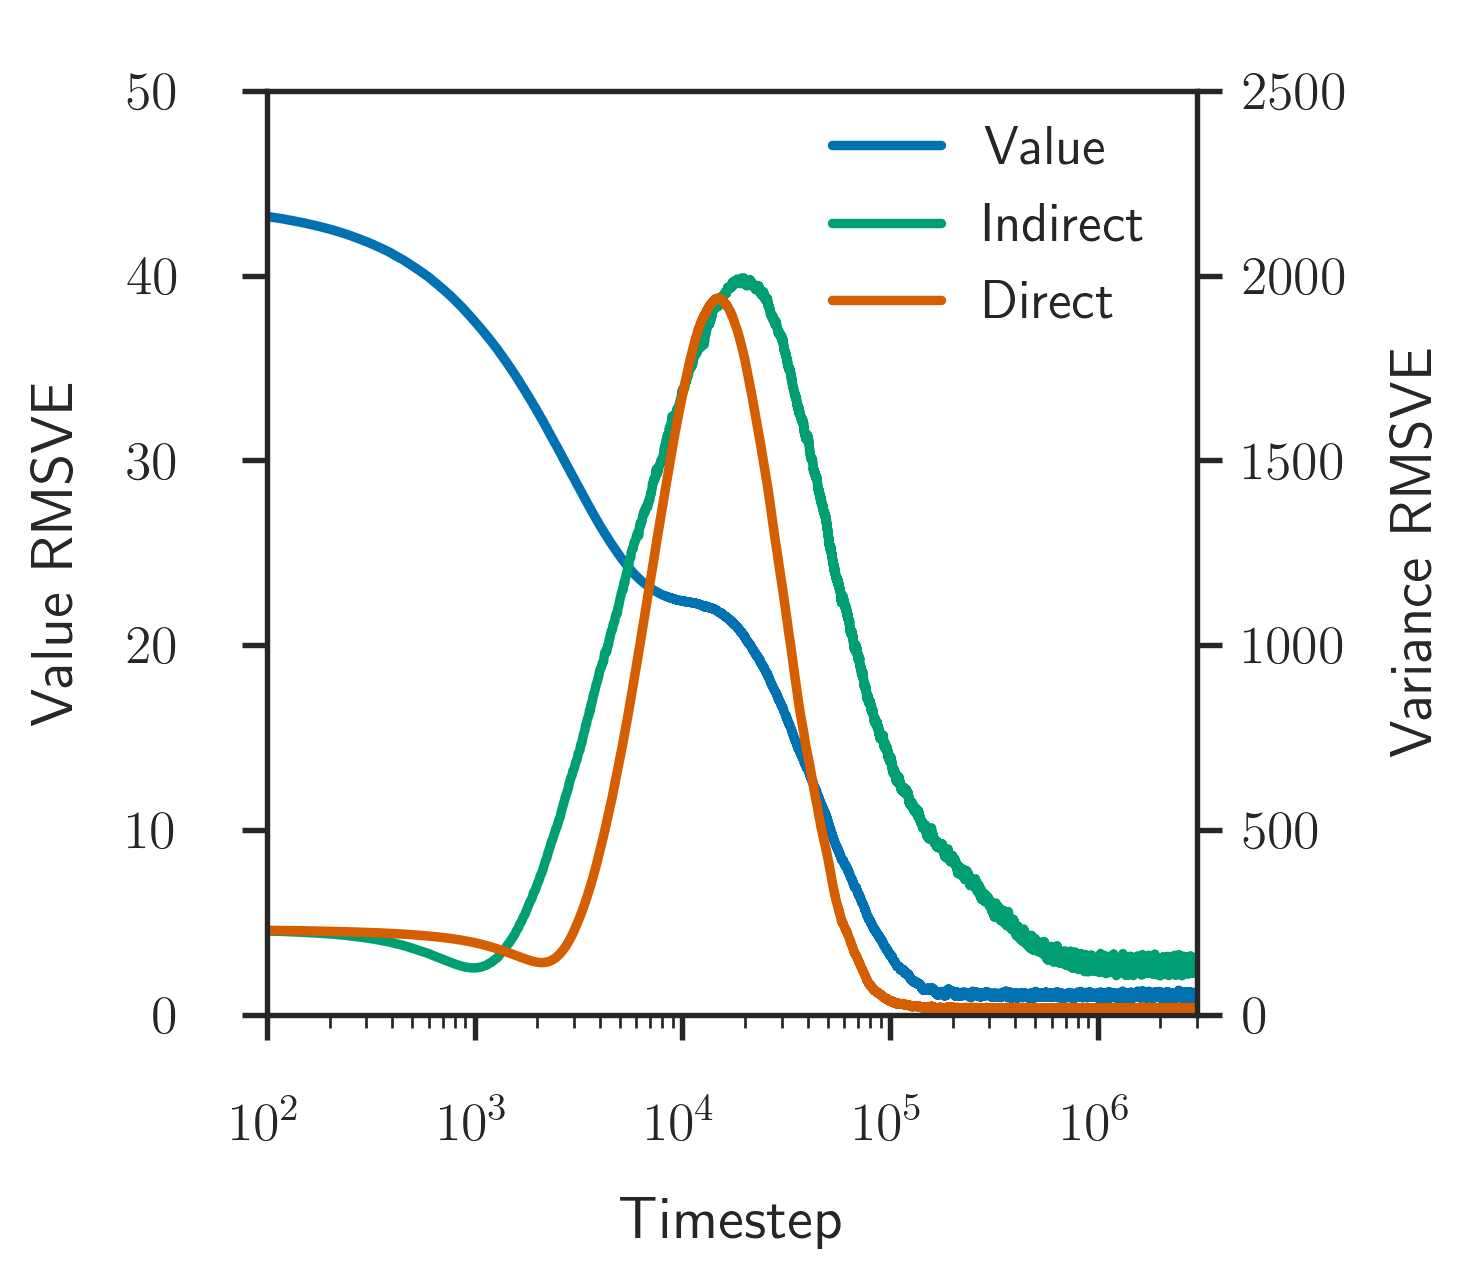
\includegraphics[height=17em]{{images/random_walk/performance.png}}
    \end{figure}
\end{frame}

\begin{frame}{What is the quality of the solutions reached?}\vspace{0.75em}
    The direct method reaches a much better fixed point and exhibits much less variance in its variance estimates:

    \vspace{0.5em}
    \begin{figure}
        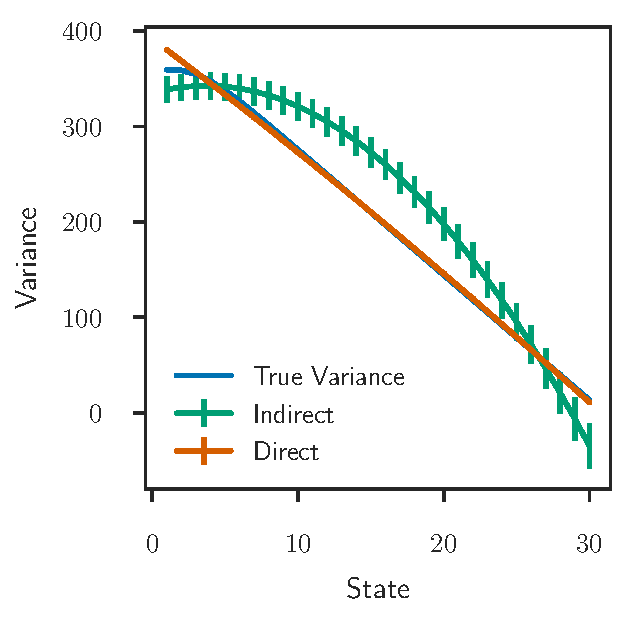
\includegraphics[height=17em]{{images/random_walk/quality.pdf}}\hspace{2.5em}
    \end{figure}
\end{frame}

\begin{frame}{What is the parameter sensitivity?}\vspace{0.75em}
    In this domain, the direct method is much less sensitive to the choice of step sizes than the indirect method:

    \vspace{0.5em}
    \begin{figure}
        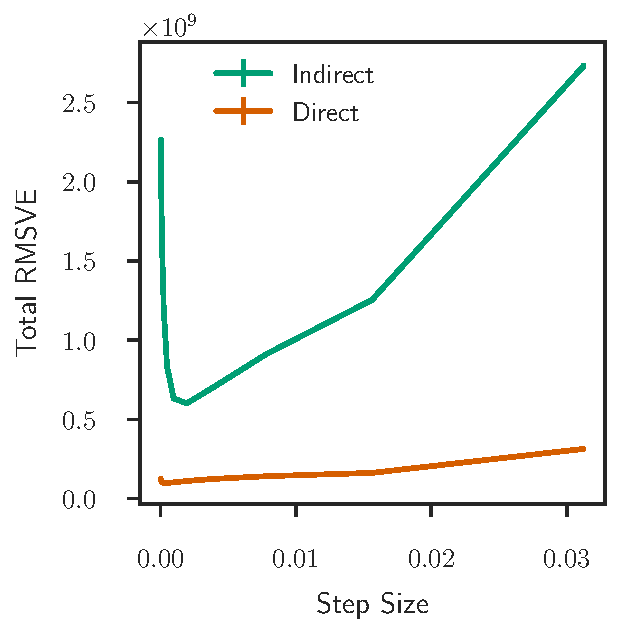
\includegraphics[height=17em]{{images/random_walk/sensitivity.pdf}}\hspace{2.5em}
    \end{figure}
\end{frame}

\begin{frame}{Summary}
    We have described a method of directly estimating the variance of the return using temporal-difference methods. We have argued that learning the variance of the return can

    \begin{itemize}
        \item tell us \alert{interesting} information about our domain,
        \item tell us \alert{useful} information about the distribution of our return, and
        \item can be used to \alert{learn} how to learn.
    \end{itemize}
\end{frame}

\begin{frame}{Summary (continued)}
    We have furthermore shown evidence that the direct method:

    \begin{itemize}
        \item learns just as fast and occasionally \alert{faster} than the indirect method,
        \item is \alert{more robust} to inconsistencies in the value and variance learner, and
        \item exhibits substantially \alert{better} performance under linear function approximation.
    \end{itemize}
\end{frame}

\plain{}{Questions?}

\end{document}
